\runningheader{Oppgave j), frivillig}{}{Side \thepage\ av \numpages}


% ********************************************************
% oppgave j) 
% ********************************************************  
\item[j)]
  Kopier modellen fra i). Siden temperaturer utenfor
  definisjonsområdet mellom  $-150^{\circ}$C til $100^{\circ}$C gir
  ufysiske tettheter skal du nå begrense verdien på det som
  sendes inn ved å benytte
  en {\sf  Saturation}-blokk som vist under
  \begin{figure}[H]
    \centering
    \hspace*{0mm}\scalebox{0.8}{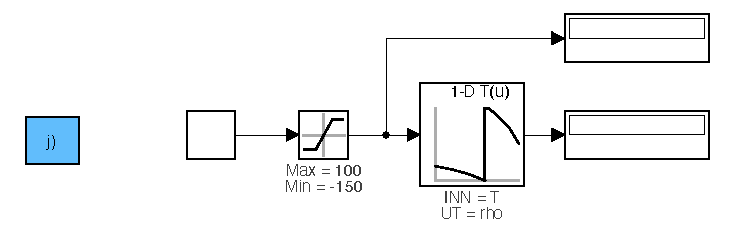
\includegraphics{2j.pdf}}
  \end{figure}
 Spesifiser nedre grense
  lik $-150$ og øvre grense lik 100, og  plasser blokken
  som vist over.

  Legg gjerne til en ny {\sf  Display}-blokk som viser hvilken verdi
  som sendes inn til {\sf 1-D Lookup table}-blokken. 
  
  Test ut med å skrive inn f.eks. $-200$, 200 eller 1000 i {\sf Constant}-blokken.

  {\color{red}La simuleringstiden fortsatt være  25 sekund.}

Ta med skjermdump av
resultatet.
